\chapter{Recurrent Neural Networks}
Molti dei dati che incontriamo nel mondo reale sono di natura sequenziale: il testo è una sequenza di parole, la musica è una sequenza di note, e i dati finanziari sono una serie temporale di valori. Lavorare con questo tipo di dati presenta una sfida unica: il significato di un elemento spesso dipende da quelli che lo precedono. Le tradizionali reti neurali feed-forward, che elaborano ogni input in maniera indipendente, non sono adatte a questo compito, poiché mancano di una "memoria" per conservare informazioni sugli eventi passati. Le \textbf{Reti Neurali Ricorrenti} (RNN) sono state progettate proprio per superare questo limite. Costituiscono una classe di architetture neurali dotate di una memoria interna che evolve nel tempo. Questa memoria consente al modello di conservare informazioni sugli stati precedenti della sequenza, rendendo possibile la modellazione delle dipendenze temporali. Tale proprietà è fondamentale in applicazioni dove il contesto è tutto, come nella traduzione automatica, nel riconoscimento vocale o nella generazione di testo. L'introduzione dello stato ricorrente permette di superare i limiti di approcci più classici, come le catene di Markov, che faticavano a catturare relazioni complesse tra eventi consecutivi.

\section{Architettura delle RNN}
Le reti neurali \textit{feedforward} elaborano gli input in un'unica direzione, dall'input all'output, senza tenere conto della sequenzialità o della dipendenza temporale dei dati. In tal modo, presuppongono che ogni input e output sia indipendente dagli altri. Questa assunzione le rende inadatte a compiti in cui il contesto o l'ordine temporale sono fondamentali (e.g traduzione, modellazione linguistica, riconoscimento vocale). Le Reti Neurali Ricorrenti (RNN), invece, sono progettate per lavorare su sequenze, riconoscendo pattern temporali grazie alla capacità di mantenere una \textit{memoria} implicita dello stato precedente della rete, grazie a un ciclo di retroazione.
\begin{figure}
    \centering
    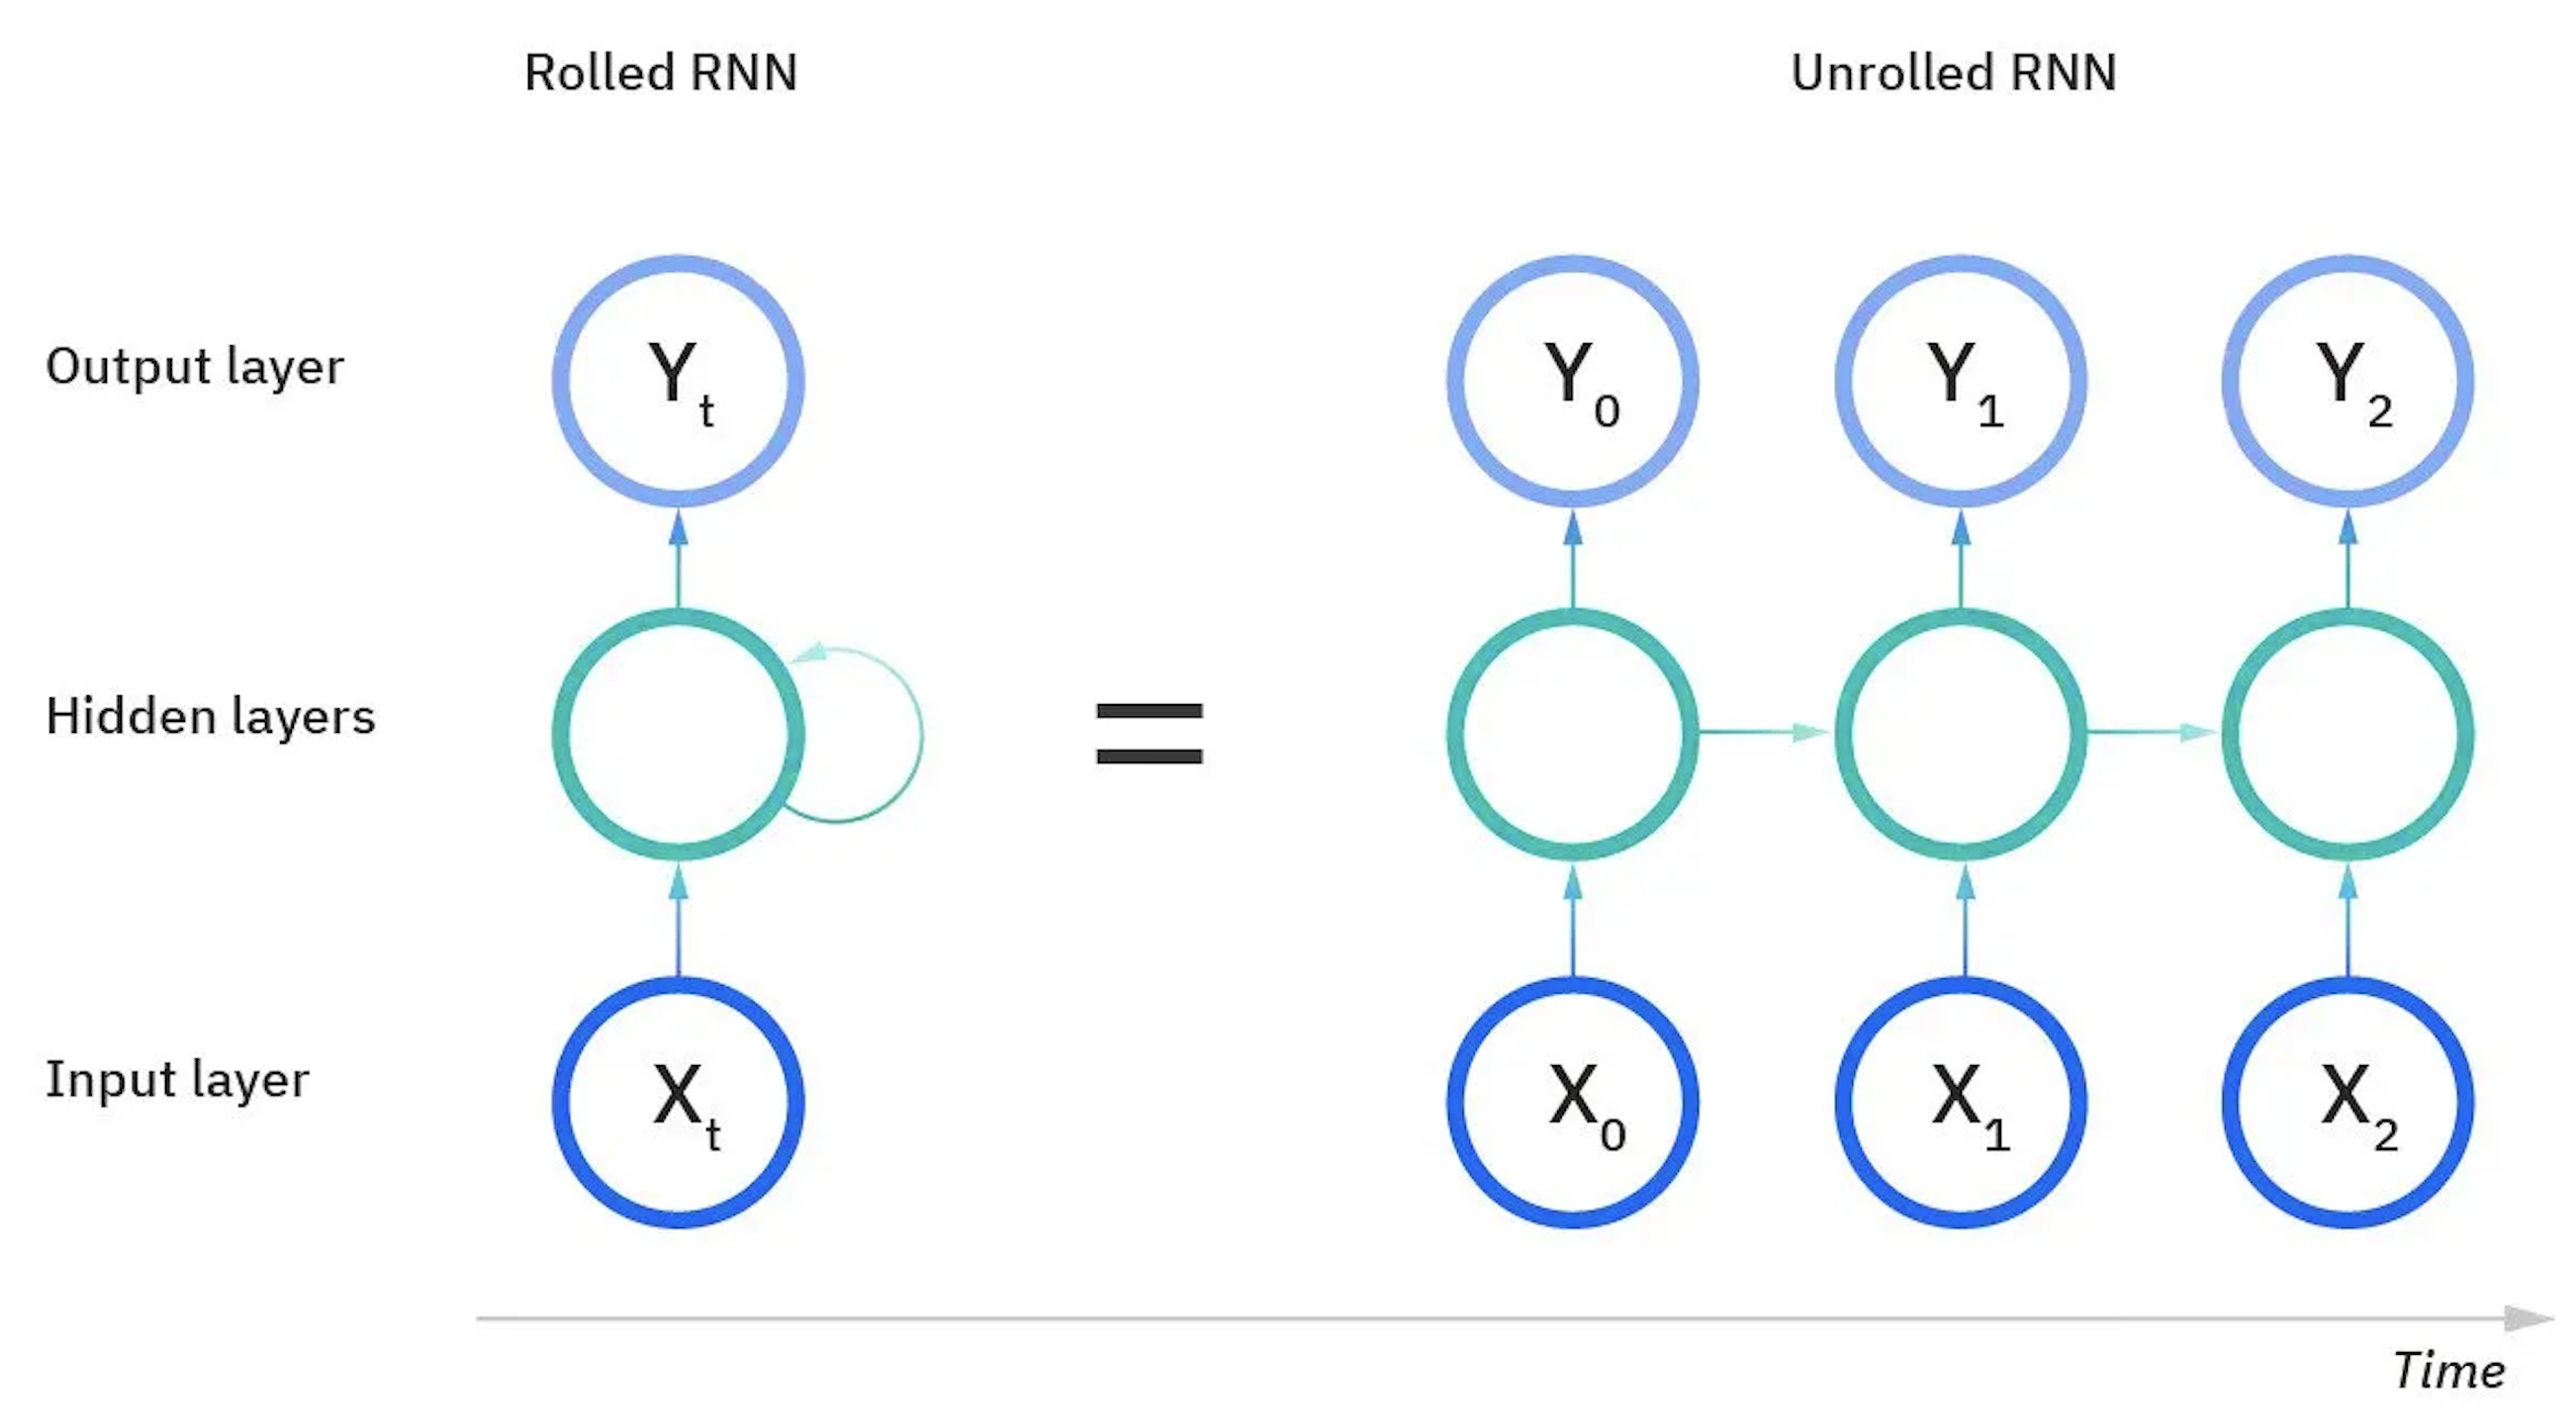
\includegraphics[width=0.70\textwidth]{figure/RNNRoll.png}
    \caption{Rappresentazione schematica di una Recurrent Neural Network, nella versione "arrotolata" (a sinistra) e "srotolata" (a destra).}
    \label{fig:rolledRNN}
\end{figure}
Considerando l'espressione idiomatica inglese "feeling under the weather", comunemente usata per indicare che qualcuno è malato. L'espressione ha senso solo se le parole vengono pronunciate in quell'ordine specifico. Una RNN è in grado di interpretarla correttamente perché, elaborando ogni parola nel contesto delle precedenti, riesce a mantenere il significato dell'intera sequenza. La vista "arrotolata" della Figura~\ref{fig:rolledRNN} rappresenta l'intera rete come una singola entità che incorpora la memoria. La vista "srotolata" invece mostra i diversi \textit{timestep}, ognuno dei quali corrisponde a un'istanza temporale della rete (e.g "Feeling", "under", "the", "weather"). Ogni nodo tiene conto dello stato nascosto accumulato nel tempo per predire il token successivo.

\subsection{La cella di ricorrenza}
La caratteristica distintiva delle RNN è la presenza di una struttura ricorsiva che consente di mantenere uno \textit{stato nascosto} (\textit{hidden state}) lungo la sequenza (Figura~\ref{fig:recurrency_cell}). A ogni istante temporale, la rete riceve l'input corrente ($x_t$) e lo stato nascosto del passo precedente ($h_{t-1}$), aggiornando lo stato attuale ($h_t$) tramite una funzione parametrizzata.
\begin{figure}
    \centering
    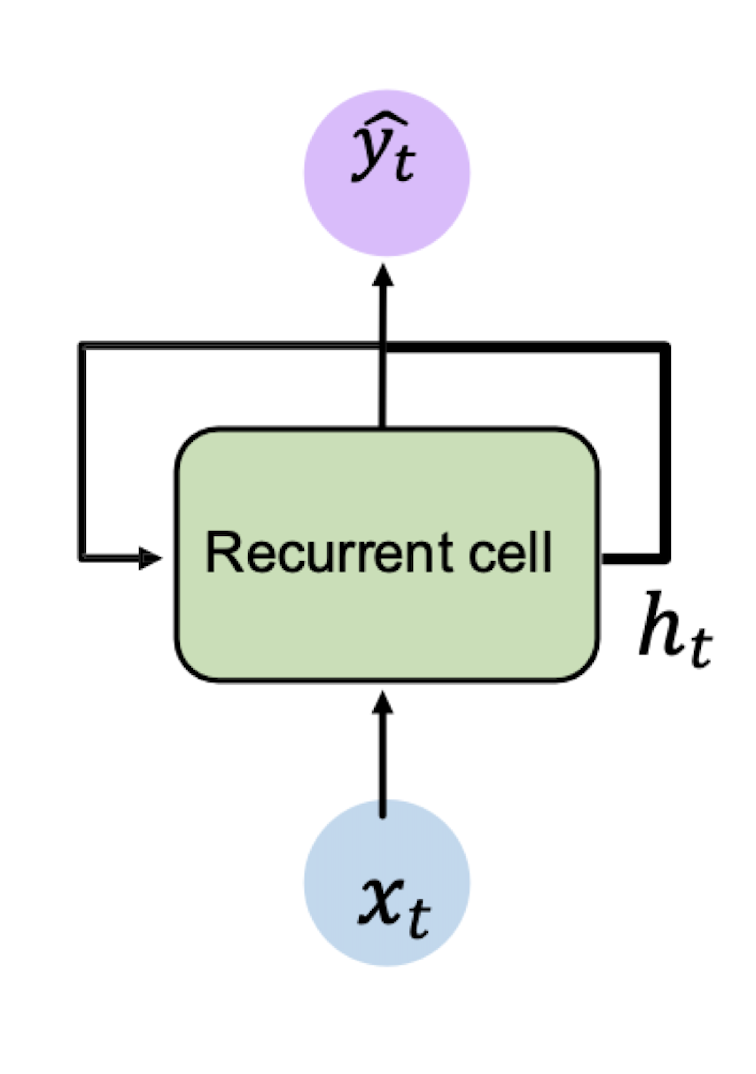
\includegraphics[width=0.32\textwidth]{figure/Recurrency_RNN.png}
    \caption{Rappresentazione della cella di ricorrenza, che integra input corrente e stato precedente attraverso la catena di retroazione.}
    \label{fig:recurrency_cell}
\end{figure}
Questo comportamento si può formalizzare tramite la seguente equazione:
\begin{equation}
    h_t = f_W(x_t, h_{t-1})
\end{equation}

Dove $f_W$ è una funzione non lineare parametrizzata dai pesi $W$. L'output della rete a un dato tempo $t$, indicato con $\hat{y_t}$, viene poi calcolato a partire dallo stato nascosto corrente $h_t$. Matematicamente, l'aggiornamento dello stato nascosto e il calcolo dell'output possono essere espressi come segue:
\begin{equation}
    h_t = \tanh(W_{hh}^T\,h_{t-1} + W_{xh}^T\,x_t) \qquad \hat{y}_t = W_{hy}^T\,h_t
\end{equation}

Un modo intuitivo per visualizzare una RNN è attraverso la sua rappresentazione "srotolata" nel tempo (Figura~\ref{fig:rolledRNN}). Sebbene la rete abbia un solo insieme di pesi ($W_{hh}$,$W_{xh}$,$W_{hy}$), possiamo immaginarla come una sequenza di copie della stessa cella, ognuna delle quali passa il proprio stato a quella successiva. Riducendo il carico computazionale rispetto a una rete profonda convenzionale e consente di modellare sequenze con efficienza. Un esempio semplificato del flusso di dati in una RNN può essere descritto dal seguente pseudocodice Python:
\vspace{0.5em}
\begin{python}
    my_rnn = RNN()
    hidden_state = [0, 0, 0, 0]

    sentence = ["I", "love", "recurrent", "neural"]
    for word in sentence:
        prediction, hidden_state = my_rnn(word, hidden_state)

    nextWordPrediction = prediction
    # >>> "networks!"
\end{python}
\vspace{0.5em}

\subsection{Modelli di sequenza}    
La modellazione temporale può variare in base al tipo di task e al modo in cui si desidera produrre l'output. In Figura~\ref{fig:seqMod} sono illustrate diverse strategie:

\begin{itemize}
    \item \textbf{Many-to-One:} intera sequenza come input e un solo output finale (e.g sentiment analysis);
    \item \textbf{One-to-Many:} un input iniziale e genera una sequenza di output (e.g image captioning);
    \item \textbf{Many-to-Many:} input e output sequenziali (e.g machine translation).
\end{itemize}

\begin{figure}
    \centering
    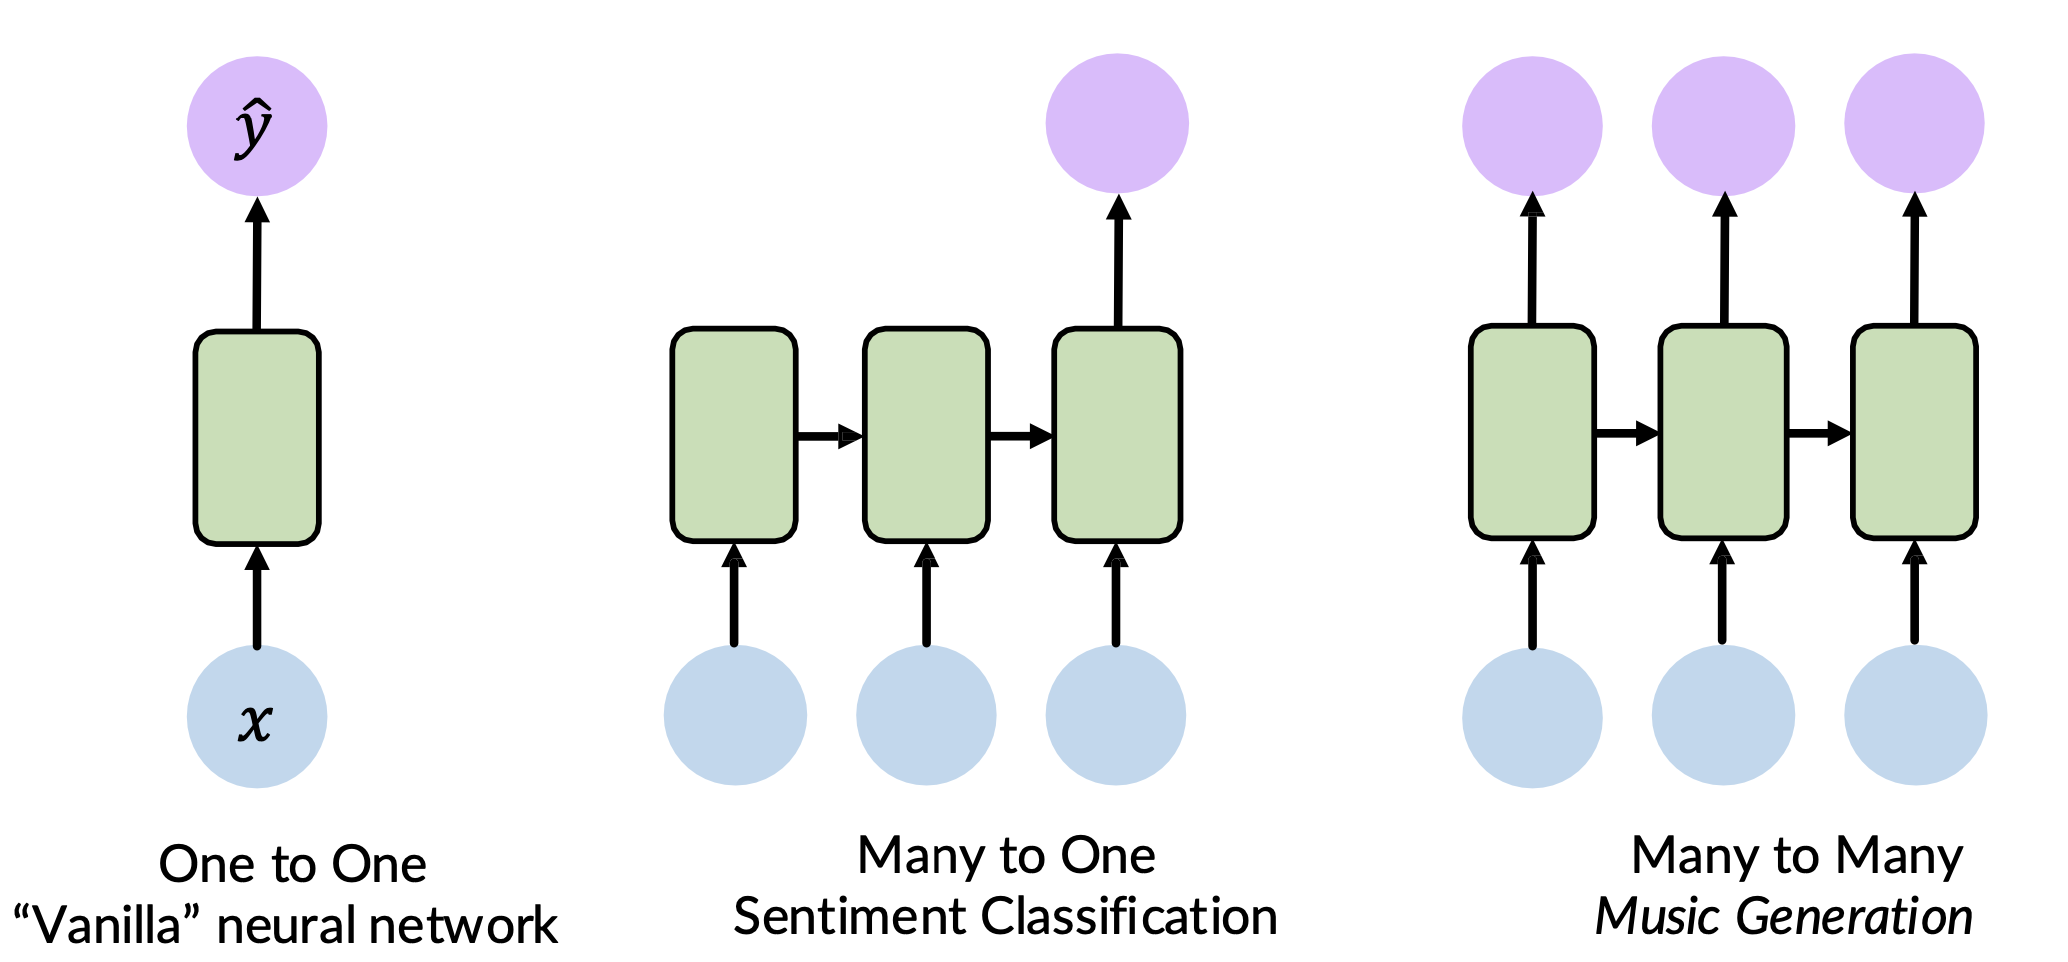
\includegraphics[width=0.85\textwidth]{figure/SequenceModeling.png}
    \caption{Esempi di modellazione della sequenza in RNN, adattabili al tipo di problema.}
    \label{fig:seqMod}
\end{figure}

\section{Rappresentare le Sequenze}
Prima di poter fornire una sequenza testuale a una RNN, dobbiamo trasformare le parole in un formato numerico che la rete possa elaborare. Esistono diversi approcci, con diversi livelli di complessità e capacità rappresentativa.
\subsection{Rappresentazioni Vettoriali}
\begin{itemize}
    \item \textbf{One-hot encoding:}Una rappresentazione semplice dove ogni parola è codificata come un vettore binario lungo quanto il vocabolario, con un solo elemento pari a 1 (in corrispondenza dell'indice della parola) e tutti gli altri a 0. Sebbene facile da implementare, questa rappresentazione è inefficiente e non cattura alcuna relazione semantica tra parole simili;
    \item \textbf{Word Embeddings:}Sono la soluzione moderna. Si tratta di rappresentazioni dense e a bassa dimensionalità dove le parole sono mappate in uno spazio vettoriale continuo. In questo spazio, parole semanticamente simili (e.g "gatto" e "cane") risultano geometricamente vicine. Questi vettori possono essere pre-addestrati su grandi corpus di testo o appresi direttamente durante l'addestramento del modello.
\end{itemize}
\subsection{Approcci Non-Ricorrenti}
\begin{itemize}
    \item \textbf{Finestra Fissa:} Una strategia che consiste nell'utilizzare solo un numero fisso n di parole precedenti per predire la successiva. Se la finestra è troppo piccola, il modello perde informazioni contestuali cruciali; se è troppo grande, diventa computazionalmente inefficiente e complesso da gestire;
    \item \textbf{Bag of Words:} In questo metodo, una frase viene rappresentata come un vettore che indica la presenza o la frequenza di ogni parola del vocabolario, ignorando completamente il loro ordine. Questo approccio perde tutta l'informazione sintattica, che è invece fondamentale per la comprensione del linguaggio. Un cambiamento nell'ordine delle parole può alterare radicalmente il significato di una frase, un aspetto che le RNN gestiscono nativamente.
\end{itemize}

La tabella di seguito riassume le caratteristiche di questi approcci:

\begin{table}[htbp]
\centering
\footnotesize
\caption{Confronto tra approcci per la rappresentazione del testo e la predizione sequenziale.}
\begin{adjustbox}{width=\textwidth}
\begin{tabular}{l|p{3.8cm}|p{3.5cm}|p{3.5cm}}
\hline
\textbf{Metodo} & \textbf{Caratteristiche principali} & \textbf{Vantaggi} & \textbf{Svantaggi} \\
\hline
\textbf{Finestra fissa} & Considera solo $n$ parole precedenti & Computazionalmente semplice & Non gestisce dipendenze a lungo termine \\
\hline
\textbf{One-hot encoding} & Rappresentazione binaria con un solo 1 attivo & Facile da implementare & Non cattura relazioni semantiche \\
\hline
\textbf{Bag of Words (BoW)} & Rappresenta la presenza o frequenza delle parole ignorando l’ordine & Semplice e interpretabile & Perde completamente l’informazione sull’ordine \\
\hline
\textbf{Word Embeddings} & Vettori densi che catturano somiglianze semantiche & Efficienza e rappresentazione semantica & Richiede training e risorse computazionali \\
\hline
\end{tabular}
\end{adjustbox}
\label{tab:metodi_sequenziali}
\end{table}

\section{Backpropagation Through Time}
L'addestramento di una RNN avviene tramite una variante dell'algoritmo di backpropagation chiamata Backpropagation Through Time (BPTT). Poiché la rete è "srotolata" nel tempo, l'errore calcolato all'ultimo passo temporale viene propagato all'indietro attraverso tutti i passi precedenti per aggiornare i pesi condivisi. Durante questo processo, il gradiente della funzione di costo rispetto ai pesi viene calcolato applicando ripetutamente la regola della catena. Lo stato nascosto $h_t$ dipende da $h_{t-1}$, che a sua volta dipende da $h_{t-2}$, e così via. Questo crea una lunga catena di moltiplicazioni di matrici Jacobiane:

\begin{equation}
    \frac{\partial L}{\partial W} = \sum_{t = 1}^T \frac{\partial L_t}{\partial h_t}\cdot\frac{\partial h_t}{\partial h_{t-1}}\cdot\cdot\cdot\frac{\partial h_1}{\partial W}
\end{equation}

\begin{figure}[!ht]
    \centering
    \begin{tikzpicture}[rnn/.style={draw, rectangle, rounded corners=5pt, minimum height=1.2cm, minimum width=1.8cm, fill=blue!10}, arrowfwd/.style={->, thick, blue}, arrowbwd/.style={->, thick, red, dashed}, every node/.style={font=\small}]

        \node[rnn] (rnn0) at (0,0) {RNN$_0$};
        \node[rnn, right=of rnn0] (rnn1) {RNN$_1$};
        \node[rnn, right=of rnn1] (rnn2) {RNN$_2$};

        \node[above=0.6cm of rnn0] (x0) {$x_0$};
        \node[above=0.6cm of rnn1] (x1) {$x_1$};
        \node[above=0.6cm of rnn2] (x2) {$x_2$};

        \node[below=0.6cm of rnn0] (y0) {$\hat{y}_0$};
        \node[below=0.6cm of rnn1] (y1) {$\hat{y}_1$};
        \node[below=0.6cm of rnn2] (y2) {$\hat{y}_2$};

        \draw[arrowfwd] (x0) -- (rnn0);
        \draw[arrowfwd] (x1) -- (rnn1);
        \draw[arrowfwd] (x2) -- (rnn2);

        \draw[arrowfwd] (rnn0) -- (rnn1);
        \draw[arrowfwd] (rnn1) -- (rnn2);

        \draw[arrowfwd] (rnn0) -- (y0);
        \draw[arrowfwd] (rnn1) -- (y1);
        \draw[arrowfwd] (rnn2) -- (y2);

        \draw[arrowbwd] (rnn2.south west) to[out=210,in=330] (rnn1.south east);
        \draw[arrowbwd] (rnn1.south west) to[out=210,in=330] (rnn0.south east);

    \end{tikzpicture}
    \caption{Illustrazione della Backpropagation Through Time (BPTT), in cui gli errori si propagano all’indietro lungo la sequenza temporale.}
\end{figure}

Questa struttura porta inevitabilmente a due problemi noti:
\begin{itemize}
    \item \textbf{Vanishing Gradient:} i gradienti si riducono esponenzialmente man mano che si propaga l’errore, impedendo l’apprendimento delle dipendenze a lungo termine;
    \item \textbf{Exploding Gradient:} i gradienti crescono esponenzialmente, destabilizzando l’addestramento.
\end{itemize}

In entrambi i casi, il modello fatica a gestire sequenze molto lunghe o con relazioni temporali distanti. Per risolvere queste problematiche, sono state introdotte le \textbf{Gated Cells}, che vedremo nella prossima sezione.

\section{Gated Cell}

Per risolvere i problemi del gradiente, sono state introdotte architetture più sofisticate che utilizzano celle con meccanismi di gate dette \textbf{Gated Cells}. L'idea è di dotare la cella di meccanismi interni che controllano attivamente il flusso di informazioni, decidendo cosa dimenticare, cosa memorizzare e cosa passare al passo successivo.

\subsection{Long Short Term Memory Networks}
Introdotte nel 1997 da Hochreiter e Schmidhuber, le Long Short-Term Memory (LSTM) sono la variante di RNN più celebre e diffusa. Una cella LSTM (Figura~\ref{fig:LSTMSchema}), è molto più complessa di una cella RNN semplice. Oltre allo stato nascosto ($h_t$), gestisce uno stato della cella ($C_t$), che agisce come un nastro trasportatore su cui le informazioni possono viaggiare quasi inalterate lungo la sequenza. In \texttt{TensorFlow}, una cella LSTM può essere facilmente implementata con il comando \texttt{tf.keras.layers.LSTM(numUnits)}. Il cuore delle LSTM sono i \textit{gate}, che regolano l'informazione tramite funzioni sigmoidi e moltiplicazioni punto a punto:

\begin{figure}
    \centering
    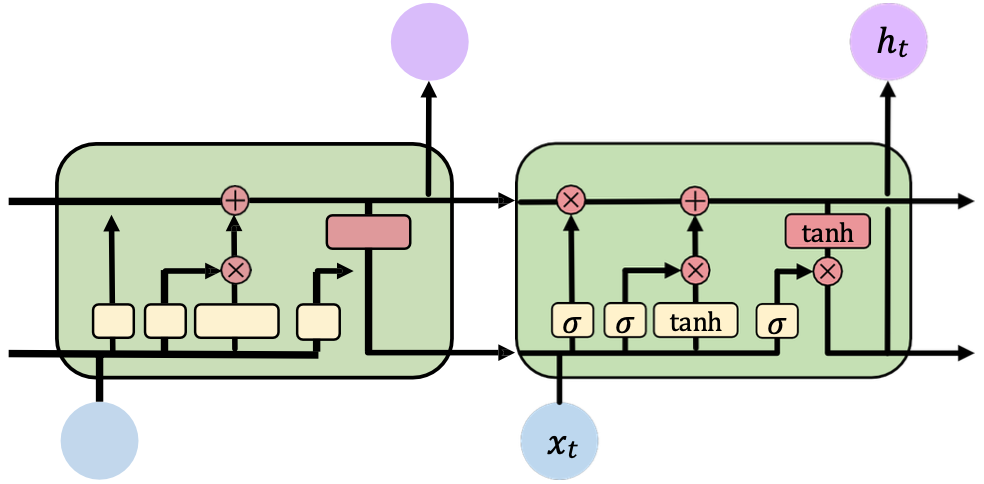
\includegraphics[width=0.85\textwidth]{figure/LSTMSchema.png}
    \caption{Rappresentazione della cella LSTM, che interagisce con un timestep precedente}
    \label{fig:LSTMSchema}
\end{figure}

\subsubsection{Forget Gate}
Il \textit{Forget Gate} decide quali informazioni dello stato precedente devono essere mantenute. Per farlo, combina l'input corrente con lo stato nascosto precedente, e li elabora tramite una funzione sigmoide. I valori prodotti, compresi tra 0 e 1, indicano il grado con cui ciascun elemento della memoria deve essere conservato: più vicino a 0 indica dimenticare, più vicino a 1 conservare.

\begin{figure}[!ht]
    \centering
    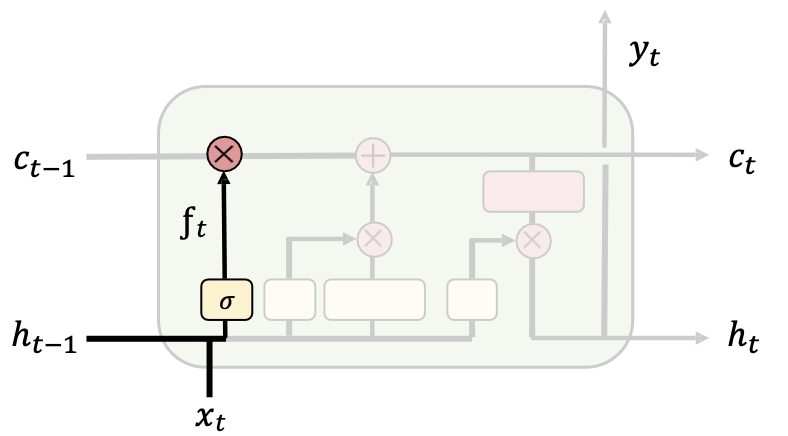
\includegraphics[width=0.55\textwidth]{figure/ForgetLSTM.png}
    \caption{Rappresentazione del gate Forget della cella LSTM}
    \label{fig:LSTMForget}
\end{figure}

\subsubsection{Store (o Input Gate)}
Lo \textit{Store Gate}, o \textit{Input Gate}, determina quali nuove informazioni devono essere aggiunte alla memoria della cella. Anche qui, l'input e lo stato nascosto precedente sono elaborati da due percorsi:
\begin{itemize}
    \item Una funzione sigmoide, che seleziona le componenti informative da aggiornare;
    \item Una funzione $\tanh$, che normalizza i nuovi valori da memorizzare in un intervallo tra -1 e 1.
\end{itemize}
Il prodotto tra questi due risultati indica quali parti della nuova informazione saranno effettivamente aggiunte allo stato interno.

\begin{figure}[!ht]
    \centering
    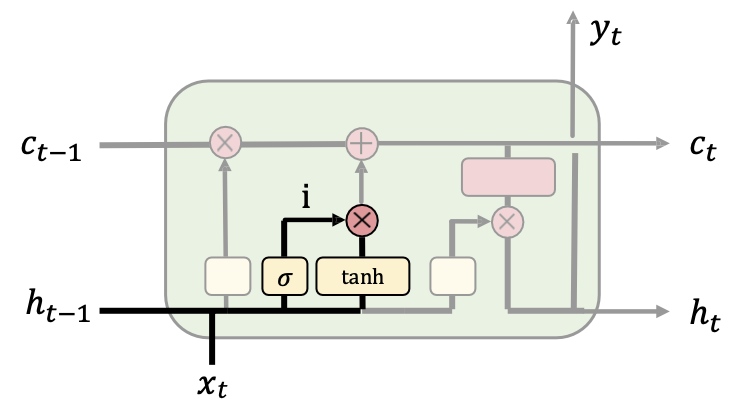
\includegraphics[width=0.55\textwidth]{figure/StoreLSTM.png}
    \caption{Rappresentazione del gate Store della cella LSTM}
    \label{fig:LSTMStore}
\end{figure}

\subsubsection{Update Gate}
L’\textit{update} rappresenta il cuore del funzionamento della LSTM. Qui lo stato della cella viene aggiornato combinando:
\begin{itemize}
    \item Lo stato precedente, pesato dal forget gate;
    \item Le nuove informazioni, selezionate dallo store gate.
\end{itemize}
La somma dei due produce il nuovo stato della cella, considerando tutti i valori che adesso la rete neurale ritiene rilevanti.

\begin{figure}[!ht]
    \centering
    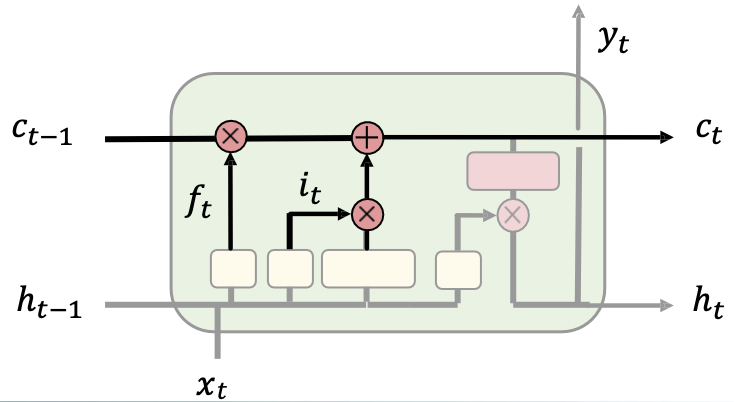
\includegraphics[width=0.55\textwidth]{figure/UpdateLSTM.png}
    \caption{Rappresentazione del gate Update della cella LSTM}
    \label{fig:LSTMUpdate}
\end{figure}

\subsubsection{Output Gate}
Infine, l’\textit{Output Gate} decide quale informazione deve essere trasmessa al prossimo timestep, ovvero il nuovo stato nascosto. L'input e lo stato nascosto precedenti vengono processati da una funzione sigmoide, mentre lo stato interno aggiornato attraversa una funzione $\tanh$. Il prodotto punto a punto di questi due risultati rappresenta l'output finale della cella.

\begin{figure}[!ht]
    \centering
    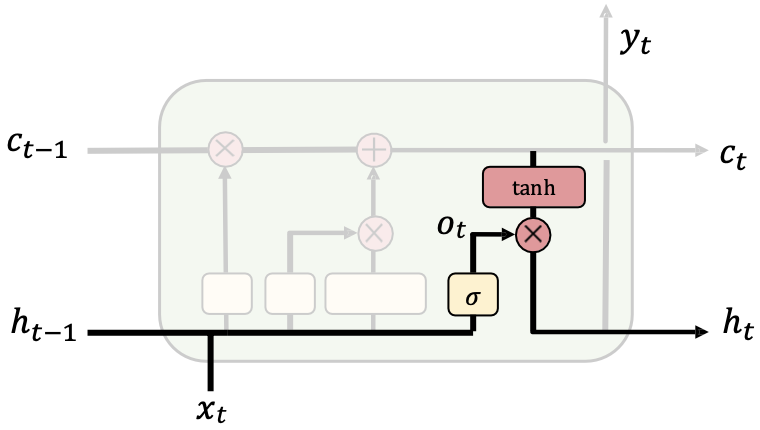
\includegraphics[width=0.55\textwidth]{figure/OutputLSTM.png}
    \caption{Rappresentazione del gate Output della cella LSTM}
    \label{fig:LSTMOutput}
\end{figure}

\subsubsection{Backpropagation solved}
Grazie a queste operazioni additive e moltiplicative, le LSTM creano dei "percorsi" attraverso i quali il gradiente può fluire senza svanire o esplodere, permettendo alla rete di apprendere dipendenze a lunghissimo termine.

\subsection{Gated Recurrent Unit}
Le Gated Recurrent Unit (GRU) sono una variante più recente e semplificata delle LSTM. Fondono lo stato della cella e lo stato nascosto in un unico vettore e utilizzano solo due gate:

\begin{itemize}
    \item \textbf{Reset Gate:} Decide quanto dello stato precedente deve essere dimenticato;
    \item \textbf{Update Gate:} Controlla quanto dello stato precedente deve essere mantenuto e quanto della nuova informazione deve essere aggiunta.
\end{itemize}
Le GRU sono computazionalmente più efficienti delle LSTM e spesso offrono performance simili, rendendole una scelta popolare in molte applicazioni.

\begin{figure}[hbtp]
    \centering
    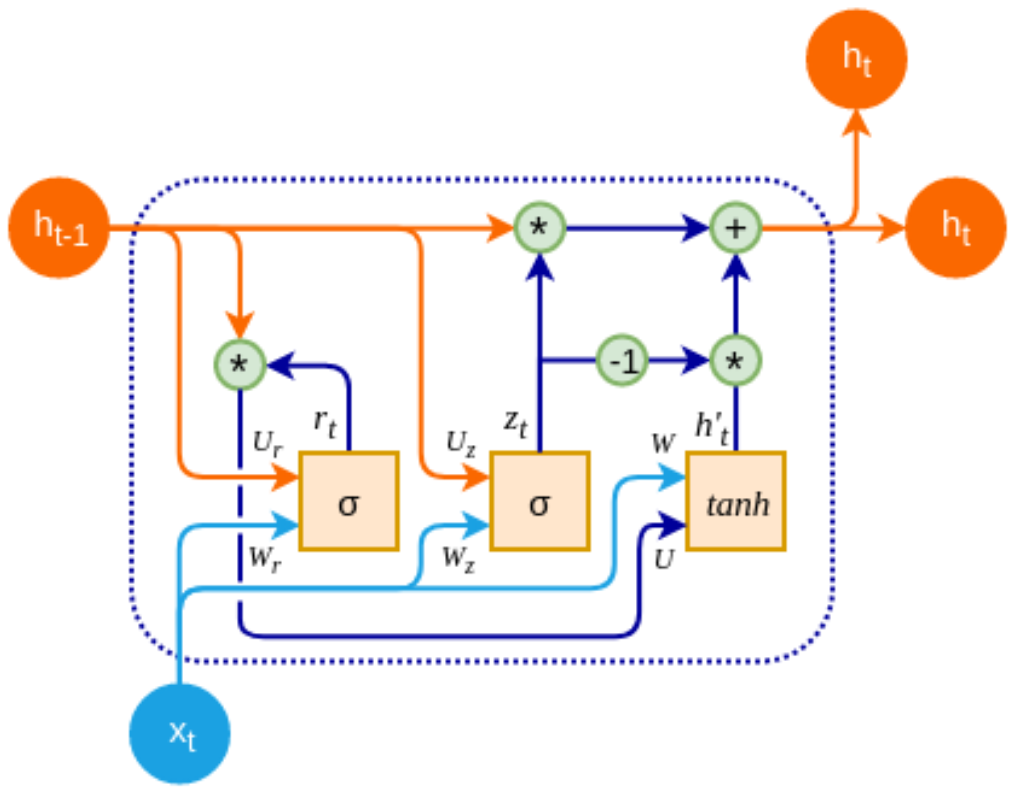
\includegraphics[width=0.60\textwidth]{figure/GNU.png}
    \caption{Rappresentazione della cella GNU, con tutti i suoi gate}
    \label{fig:GNU}
\end{figure}

\subsection{Bi-LSTM}
In molti compiti, come la traduzione o l'analisi di un testo, per comprendere il significato di una parola è utile conoscere non solo il contesto che la precede, ma anche quello che la segue. Le RNN Bidirezionali (Bi-LSTM) risolvono questo problema elaborando la sequenza in due direzioni contemporaneamente:

\begin{enumerate}
    \item Una LSTM forward processa la sequenza dall'inizio alla fine;
    \item Una LSTM backward processa la sequenza dalla fine all'inizio.
\end{enumerate}

Gli stati nascosti delle due reti vengono poi concatenati a ogni passo temporale, fornendo una rappresentazione ricca che tiene conto sia del passato che del futuro.
\begin{figure}
    \centering
    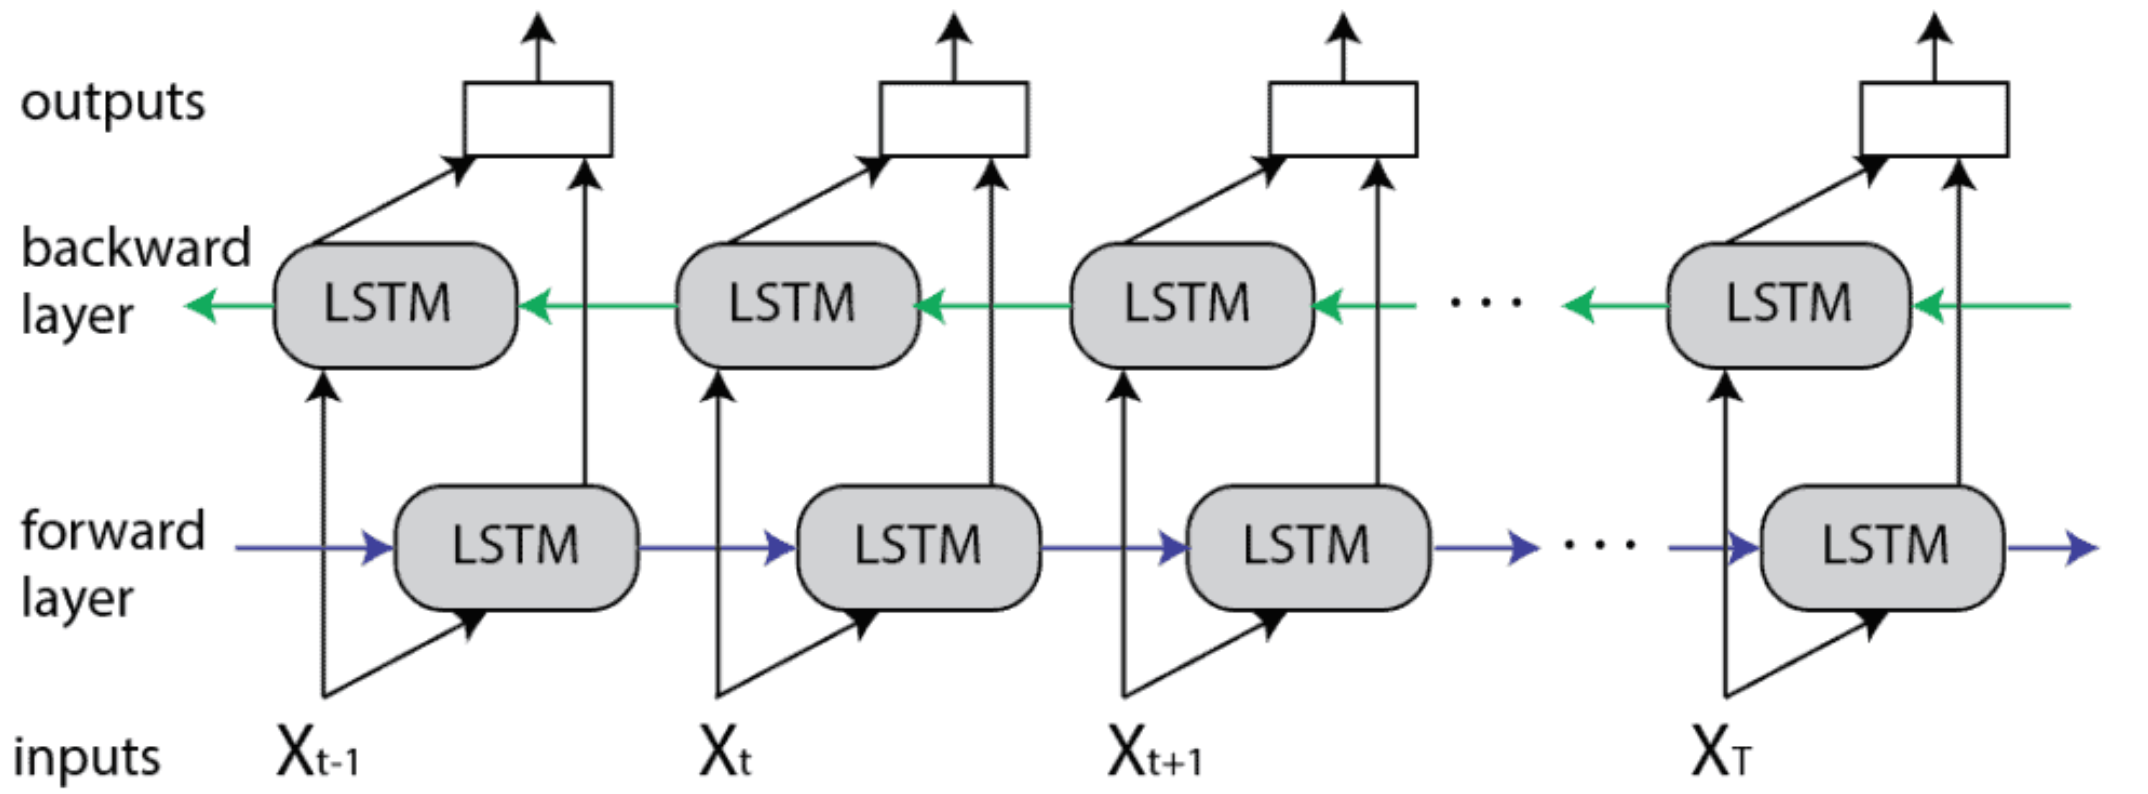
\includegraphics[width=0.8\textwidth]{figure/Bi-LSTM.png}
    \caption{Architettura di una Bi-LSTM, che elabora la sequenza in entrambe le direzioni.}
    \label{fig:bilstm}
\end{figure}
Questa potenza ha un costo: due reti LSTM devono essere addestrate simultaneamente, il che comporta un maggiore uso di memoria e tempi di addestramento più lunghi.

\subsection{Il Meccanismo dell'Attenzione}

Un limite intrinseco delle architetture encoder-decoder basate su RNN è che devono comprimere l'intera sequenza di input in un unico vettore di contesto di dimensione fissa. Questo diventa un collo di bottiglia per sequenze molto lunghe. Il \textbf{meccanismo di attenzione} (attention mechanism), che approfondiremo in seguito, risolve questo problema in modo brillante. Invece di affidarsi a un singolo vettore di contesto, l'attenzione permette al modello di "guardare indietro" all'intera sequenza di input a ogni passo della generazione dell'output, e di decidere dinamicamente su quali parti concentrarsi. Assegna un "punteggio di attenzione" a ogni stato nascosto dell'input, indicando quanto è rilevante per predire l'output corrente. Questo non solo migliora drasticamente le performance, specialmente nella traduzione automatica, ma rende anche il modello più interpretabile: possiamo visualizzare su quali parole di input il modello si sta "concentrando" per produrre una certa parola di output.

\begin{figure}
    \centering
    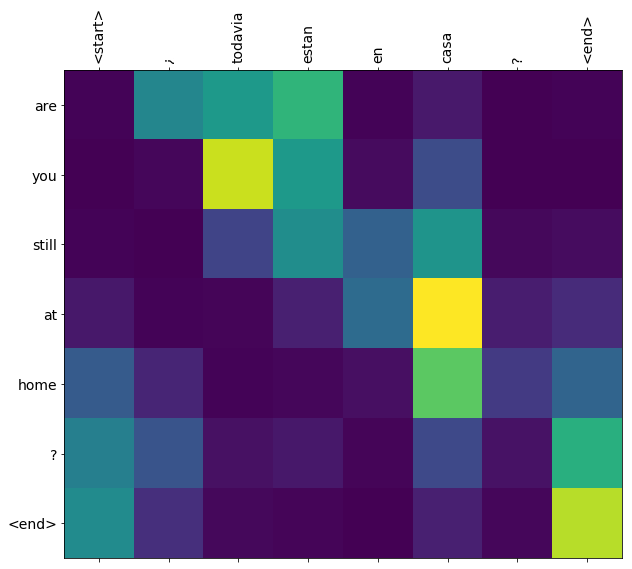
\includegraphics[width=0.40\textwidth]{figure/AttentionEx.png}
    \caption{Rappresentazione del meccanismo dell'attenzione in un compito di traduzione: le zone più gialle indicano alta probabilità di corrispondenza tra parole.}
    \label{fig:AttEx}
\end{figure}

\subsection{Bi-LSTM con Attenzione}
Un limite delle Bi-LSTM è che, nonostante processino la sequenza in entrambe le direzioni, alla fine restituiscono un singolo vettore che riassume l'intera sequenza. Questo può essere problematico se la sequenza è molto lunga o se alcune parti sono più rilevanti di altre. Il \textbf{meccanismo dell'attenzione} risolve questo problema: assegna un peso $\alpha_t$ a ciascun passo temporale, indicando quanto ogni stato nascosto deve contribuire all'output finale.

\begin{figure}[hbtp]
    \centering
    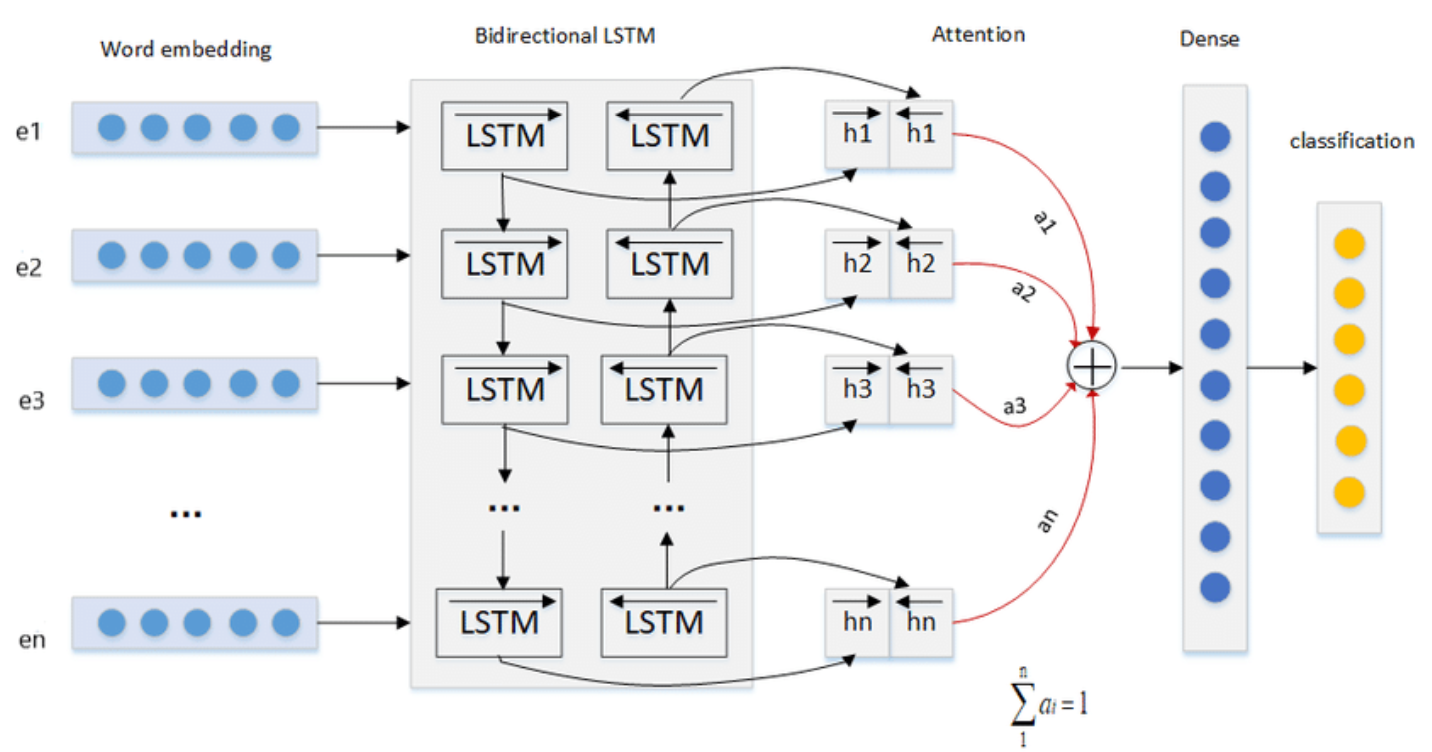
\includegraphics[width=0.8\textwidth]{figure/Bi-LSTMAtt.png}
    \caption{Architettura di una Bi-LSTM con meccanismo di attenzione}
    \label{fig:bilstmatt}
\end{figure}

In sintesi, la Bi-LSTM cattura un contesto locale e posizionale ricco per ogni parola, mentre l'attenzione impara le relazioni a lungo termine e le dipendenze globali, permettendo al modello di concentrarsi selettivamente. Questa combinazione rappresenta una delle architetture ricorrenti più performanti per compiti complessi di NLP come la traduzione automatica, la classificazione del testo e il question answering.

\subsection{Campi di Applicazione}
Grazie alla loro capacità di modellare le dipendenze temporali, le RNN e le loro varianti (LSTM, GRU, con attenzione) sono diventate lo strumento d'elezione in innumerevoli campi di applicazione dell'Intelligenza Artificiale, tra cui:
\begin{itemize}
    \item \textbf{Elaborazione del Linguaggio Naturale (NLP):} Traduzione automatica, riassunto di testi, analisi del sentimento, chatbot e generazione di testo;
    \item \textbf{Riconoscimento Vocale:} Trascrizione dell'audio parlato in testo;
    \item \textbf{Generazione di Musica:} Composizione di melodie e armonie;
    \item \textbf{Analisi di Serie Temporali:} Previsioni finanziarie, meteorologiche e monitoraggio di segnali biomedici;
    \item \textbf{Computer Vision:} Generazione di descrizioni per immagini (image captioning) e analisi di video.
\end{itemize}